\section{Introduction}
\setcounter{subsection}{0}
\renewcommand*{\thesubsection}{\Alph{subsection}.}

\paragraph*{}
Chain Replication~\cite{van2004chain} provides a storage system that is capable of supporting the following operations: store, query, and update objects. In managing distributed resources, some trade off might need to be considered, such as reserving consistency often needs to sacrifice throughput which later triggers some debates among system designers. This design claims to provide strong consistency while keeping high throughput and availability.

\paragraph*{}
Figure~\ref{fig:CRP} shows Chain Replication Protocol. It works like a linked-list that each node connects to at most two nodes so called predecessor and successor. One end of the chain is the head and another one is the tail. The head is responsible for receiving update requests; whereas the tail is responsible for receiving queries and replies (including replies for update requests). The middle nodes only forward messages from one node to the other node and cannot receive any requests from clients. Under this scenario, anything written in the tail, the data must be written in any other nodes as well - hence it has a strong consistency.
%  There is also an observer called master which controls node transitions if a failure happens such as removing, adding, and promoting a node due to a failure detection. The master server is also a subject of failure where if it fails, then the service will be stuck. Hence, the paper assumes that the master server never fails and, in practice, one may use Paxos to keep the master server up and running.

\begin{figure}[h]
    \centering
    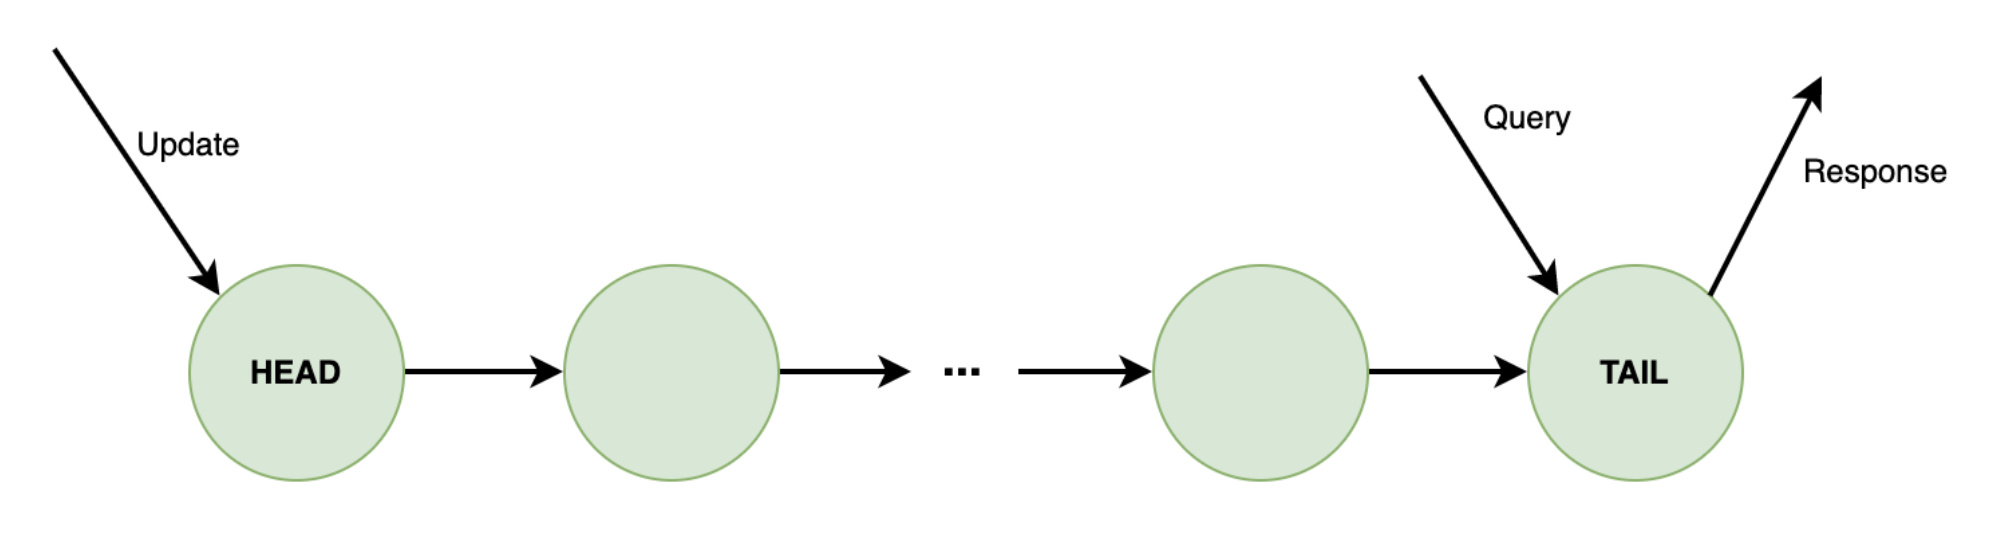
\includegraphics[width=0.8\textwidth]{images/ChainReplication.png}
    \caption{Chain Replication Protocol}
    \label{fig:CRP}
\end{figure}

\paragraph*{}
In a high level detail, each node in the protocol will keep three attributes: $Hist_{objID}$, $Pend_{objID}$, and $Sent_i$. Any request whose the $id$ is stored in $Hist_{objID}$ has been processed, otherwise it will be queued in $Pend_{objID}$. $Sent_i$ is a collection of sync requests from a node to node $i$ as a bookkeeping that node $i$ has not acknowledged those requests. To these extents, we know that
$$Hist_{objID}^j \preceq Hist_{obdID}^i$$ for some $i$, $j$ such that $i \leq j$, which is later called \textit{Update Propagation Invariant}. We also notice that when a message has been sent out of a node, that does not mean that the message will immediately arrive at the destination node, assuming that they use best-effort networking protocol. This invariant is then called as \textit{In-process Request Invariant} such that
$$Hist_{objID}^i = Hist_{objID}^j + Sent_i$$

\paragraph{}
We will use TLA+ as the formalization tool to ensure that this protocol works properly as intended, including the behavior of Update Propagation Invariant and In-process Request Invariant. We will also investigate its behavior towards server failures and ensure the objects' consistency. 
% Node failures can happen in various places (head, tail, or middle nodes), and  the protocol has different recovery reaction to which location the failed node exists.


